%!TEX root = ../my_thesis.tex
\section{Test of the decay-time fit via a toy tagger}
\label{app:toytagger}

The \emph{toy tagger} used to perform the test mentioned in Sec.~\ref{sec:mcbootstrap} is created as follows. First, a mistag ($\eta$) PDF is created from the \emph{sWeighted} $\eta$ distribution of the OS tagger on data. This template is created as a \texttt{RooHistPdf}. Then, for each candidate in each bootstrapped Monte Carlo sample, a value of $\eta$ is drawn from this PDF. The decision of the toy tagger is initially taken from the true ID of the $\Bz$ meson, which is always correct by definition. In order to emulate wrong tagging decisions, a random number $r_i$ is generated for the $i^{th}$ $\Bz$ candidate between $0$ and $1$. If $\eta_i$ is the mistag assigned to this candidate, the tagging decision $d_i$ may need to be flipped (and thus made wrong) according to the following criterion:
\begin{equation}
  d_i \to \begin{cases} -d_i &\text{if $r_i\leq\eta_i$} \\ d_i &\text{otherwise} \end{cases}. 
\end{equation}
During the time fit, the mistag calibration is simply taken as a linear function (Eq.~\ref{eq:FTcalibration}) with $p_0=\langle\eta\rangle=0.370029$ (taken from the adopted template) and $p_1=1$, which means $\omega=\eta$ for all candidates. In fact, the per-event mistag $\eta$ is the true mistag $\omega$ probability by construction. In this way, it possible to test the time fit with a per-event mistag without relying on any approximation or uncertainty coming from the calibration procedure. Moreover, the tagging efficiency is $100\%$ by construction. 

The distributions of the fitted value, error, pull and residual for the relevant parameters are shown in Fig.~\ref{fig:mc_bootstrap_decay_toytagger}. All pull distributions have means compatible with $0$ and widths compatible with $1$, meaning that the maximum likelihood estimation of the parameters is unbiased and returns correct uncertainties.

\begin{figure}[t]
        \begin{center}
                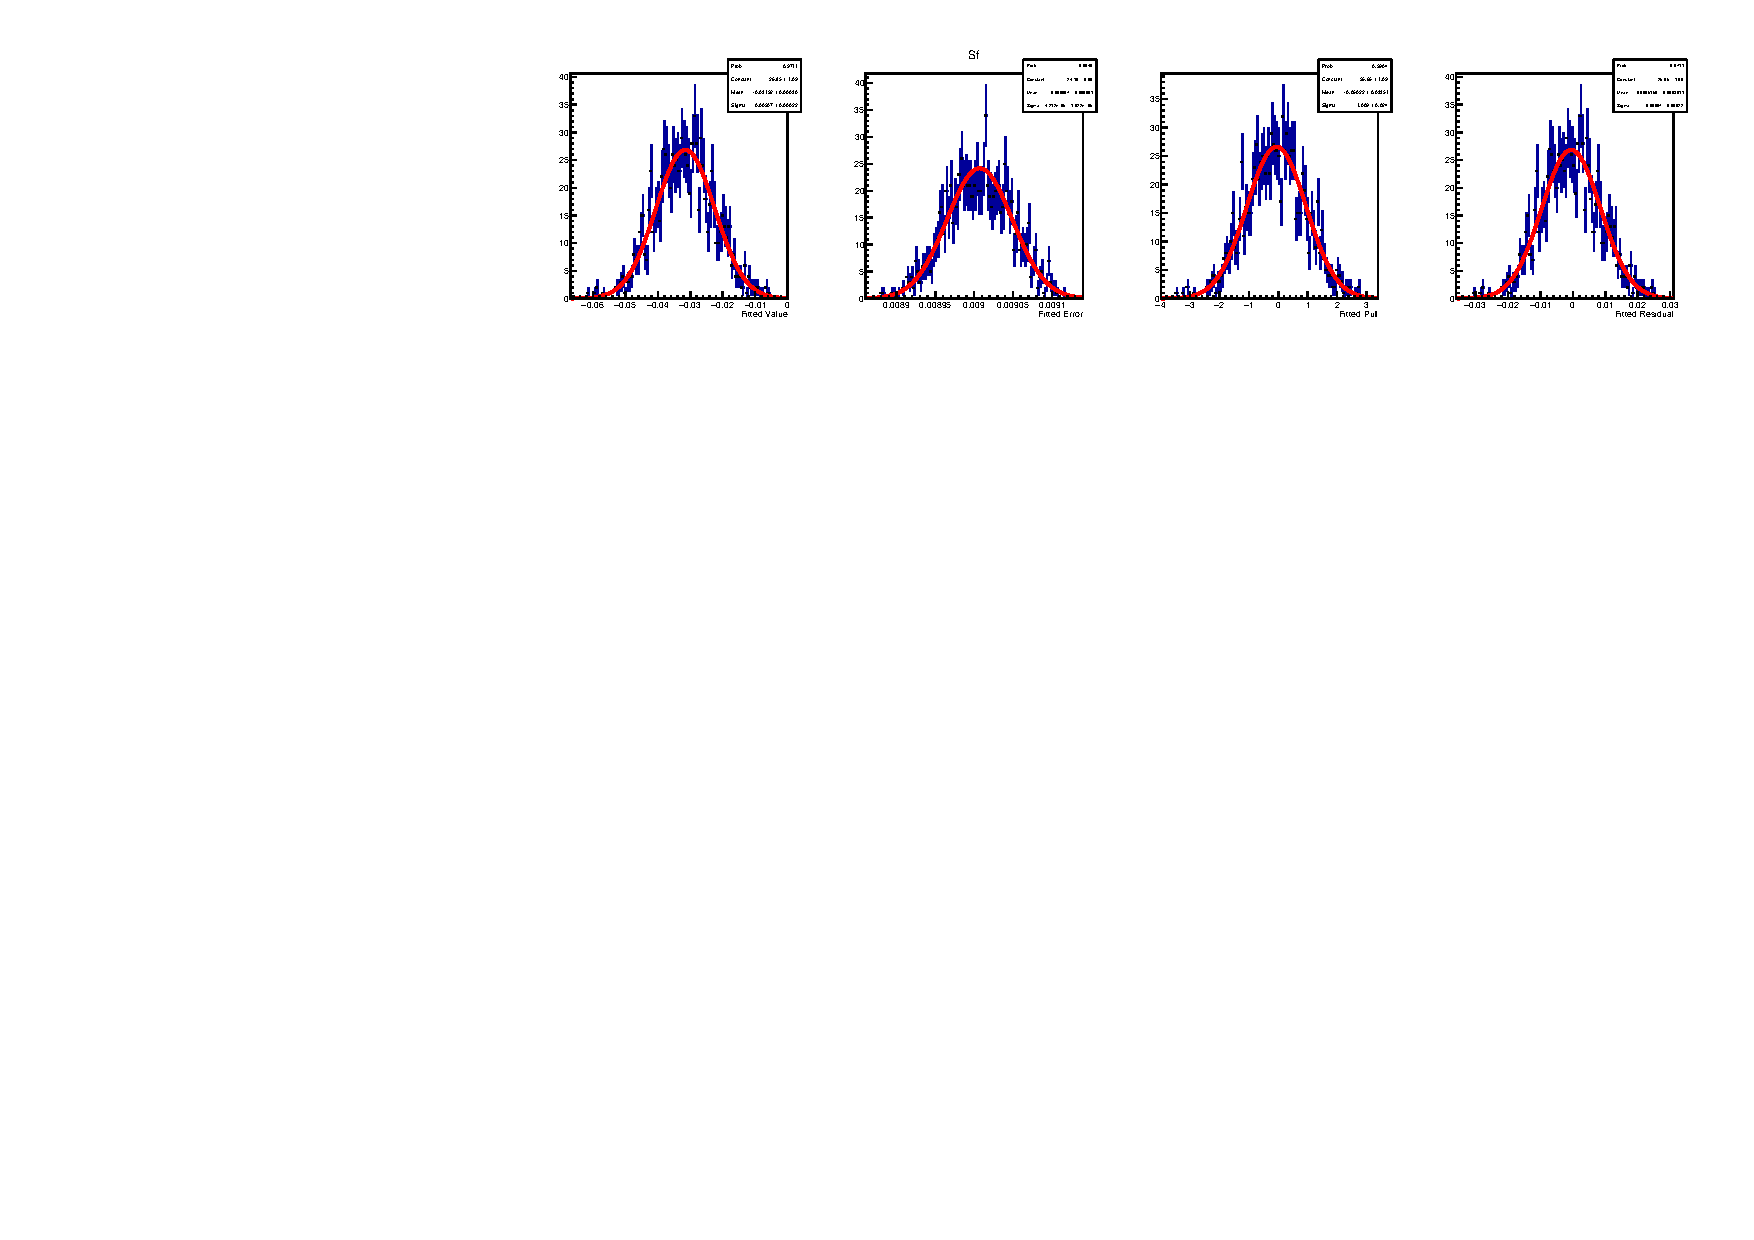
\includegraphics[width=0.9\textwidth]{AA-Appdx-toytagger/figs/1DPullPlot_Sf_SSbarAccAsymmFloatDMGammaConstrAllSamplesToyTagger.pdf} \\
                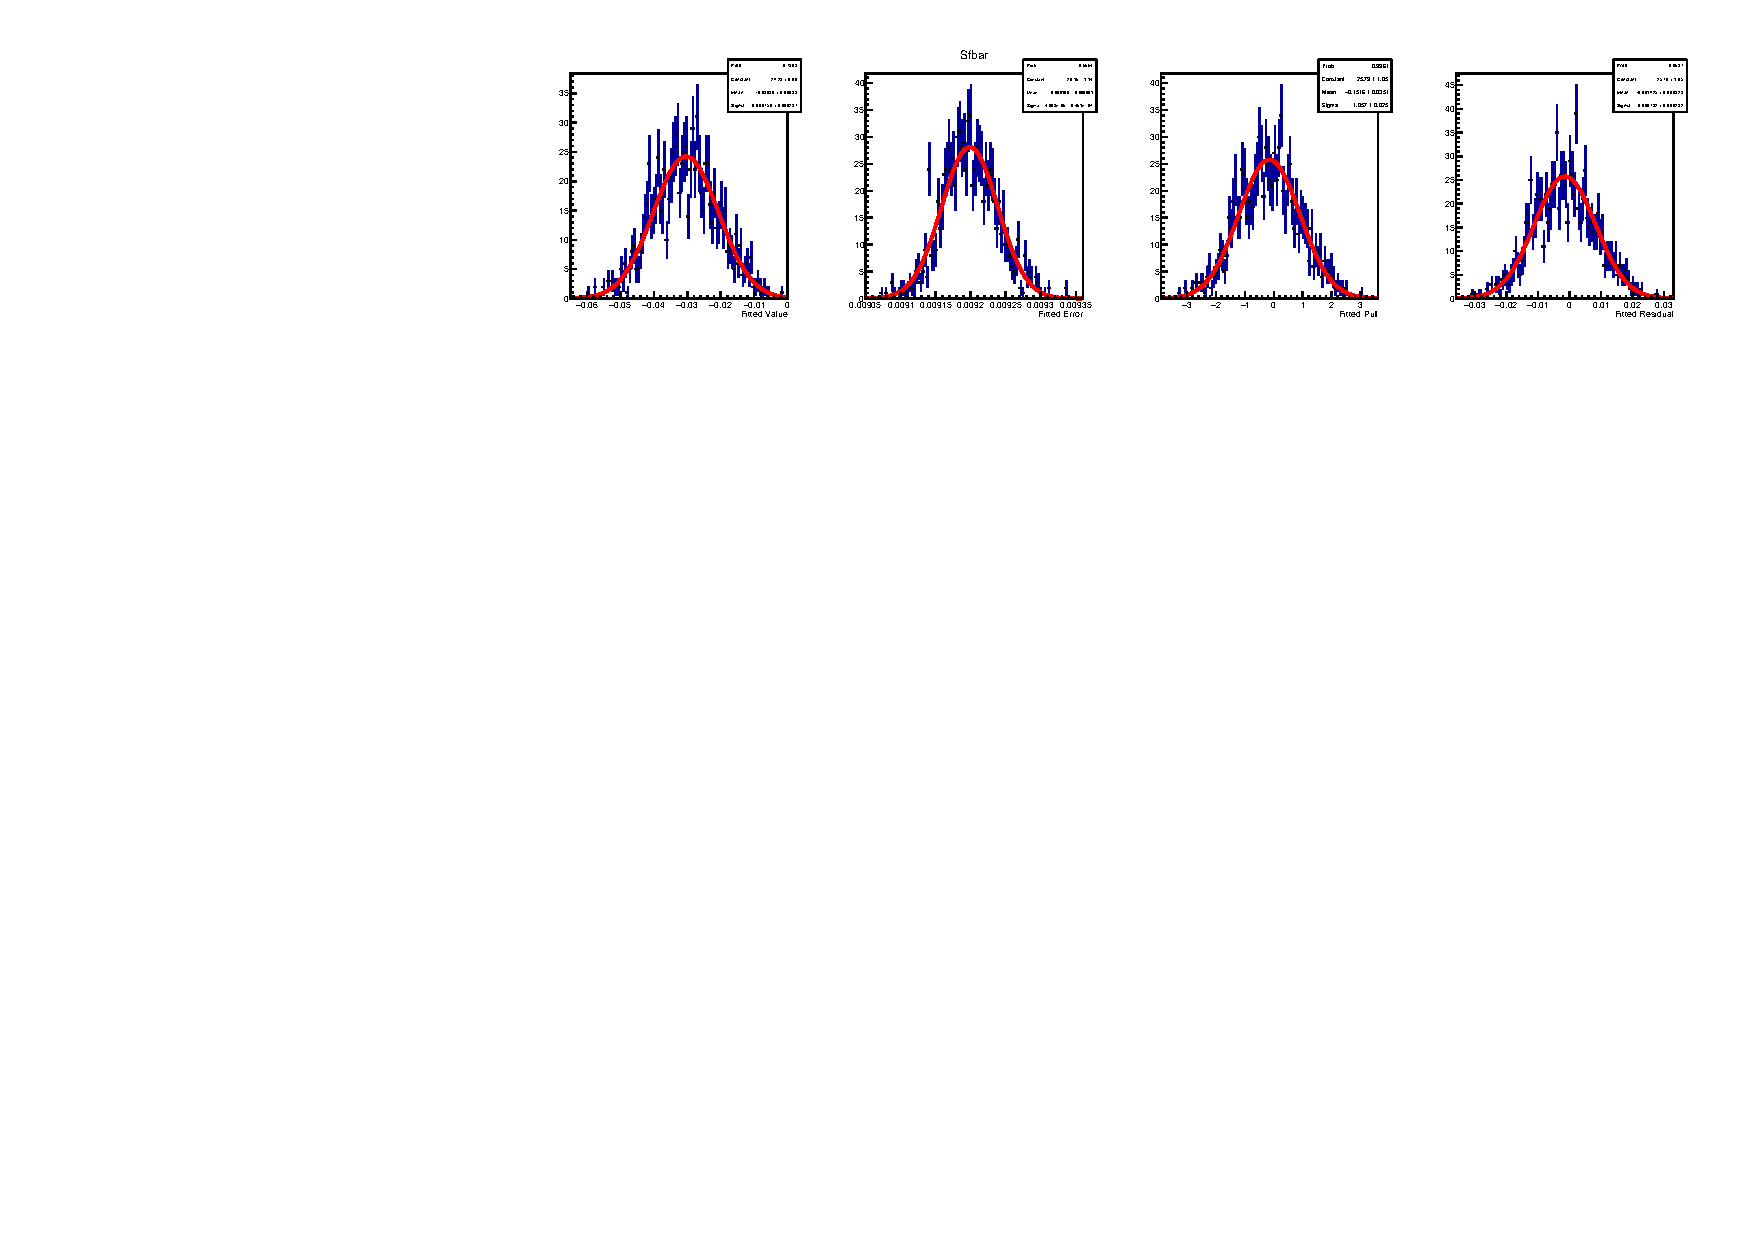
\includegraphics[width=0.9\textwidth]{AA-Appdx-toytagger/figs/1DPullPlot_Sfbar_SSbarAccAsymmFloatDMGammaConstrAllSamplesToyTagger.pdf} \\
                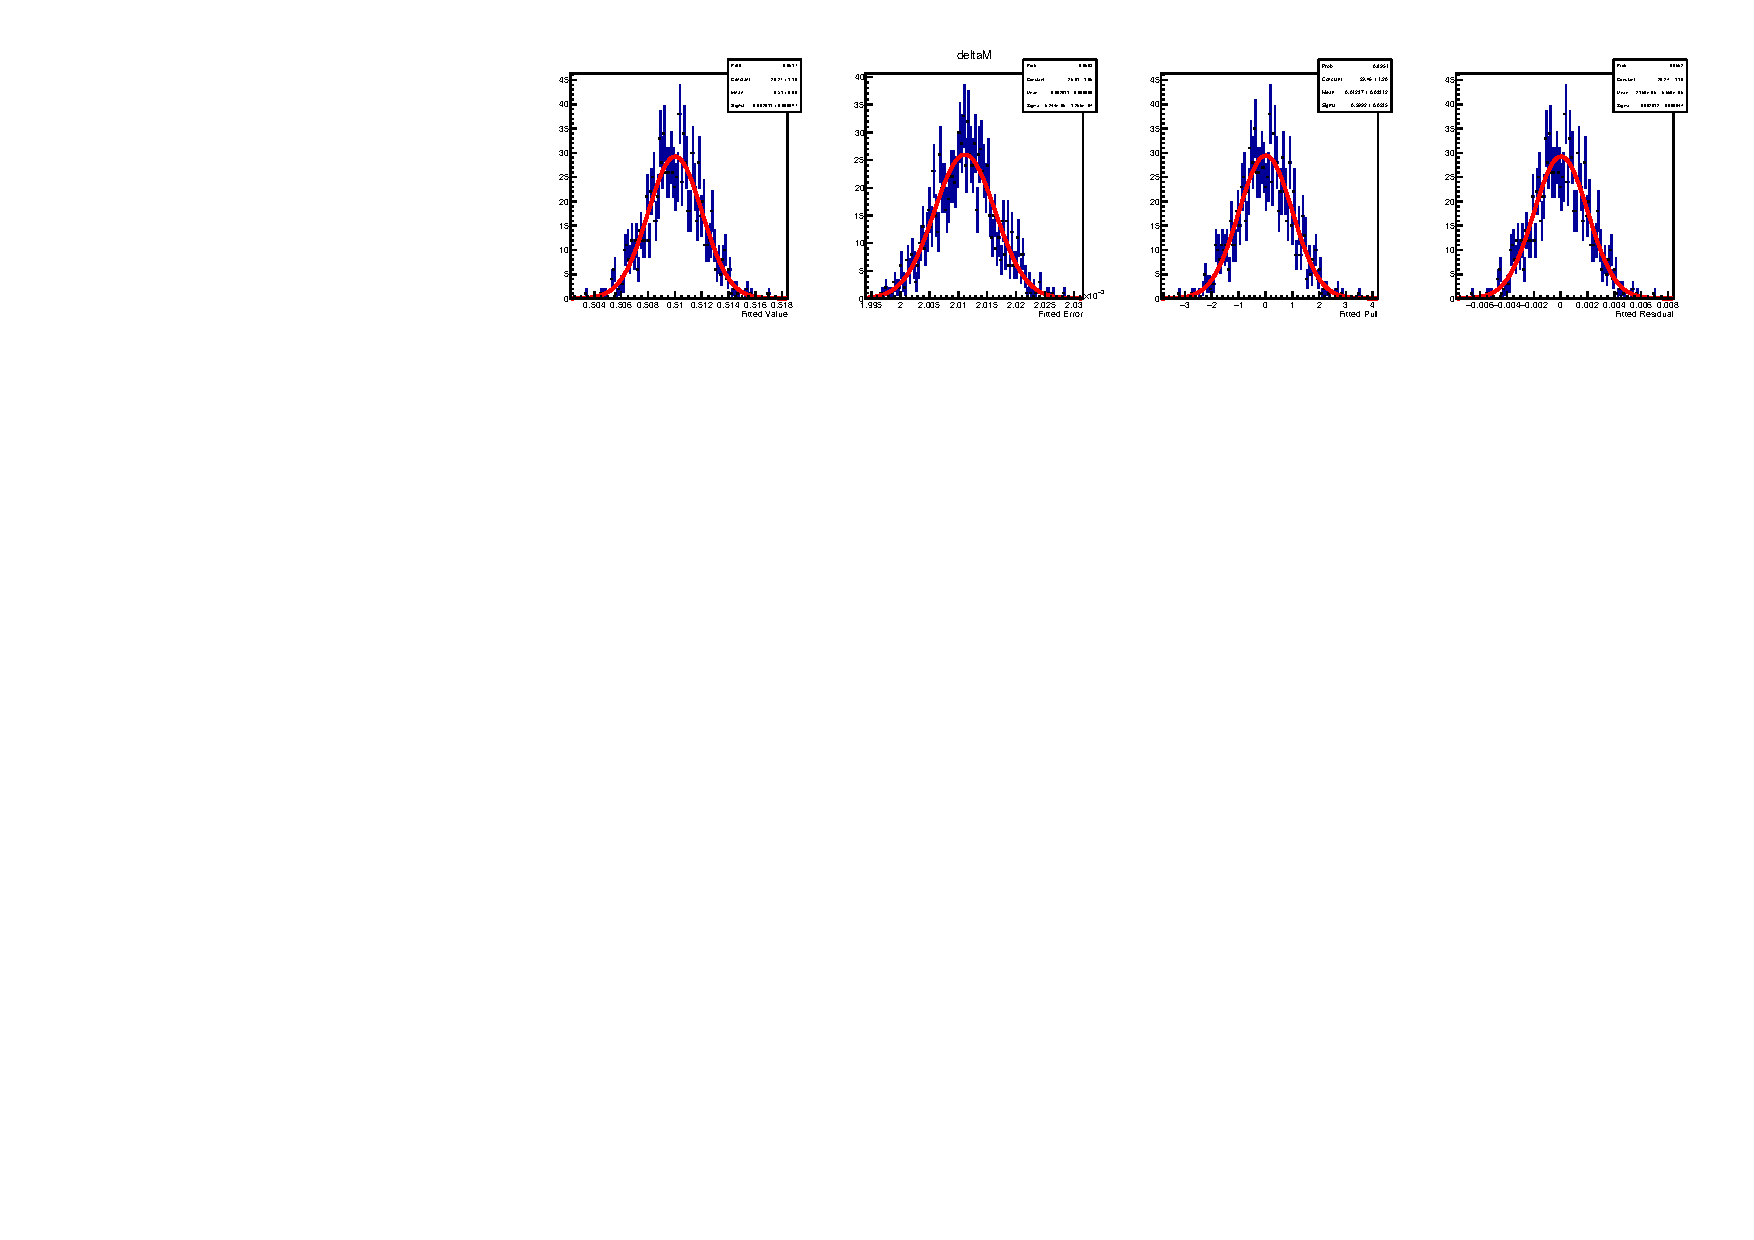
\includegraphics[width=0.9\textwidth]{AA-Appdx-toytagger/figs/1DPullPlot_deltaM_SSbarAccAsymmFloatDMGammaConstrAllSamplesToyTagger.pdf} \\
                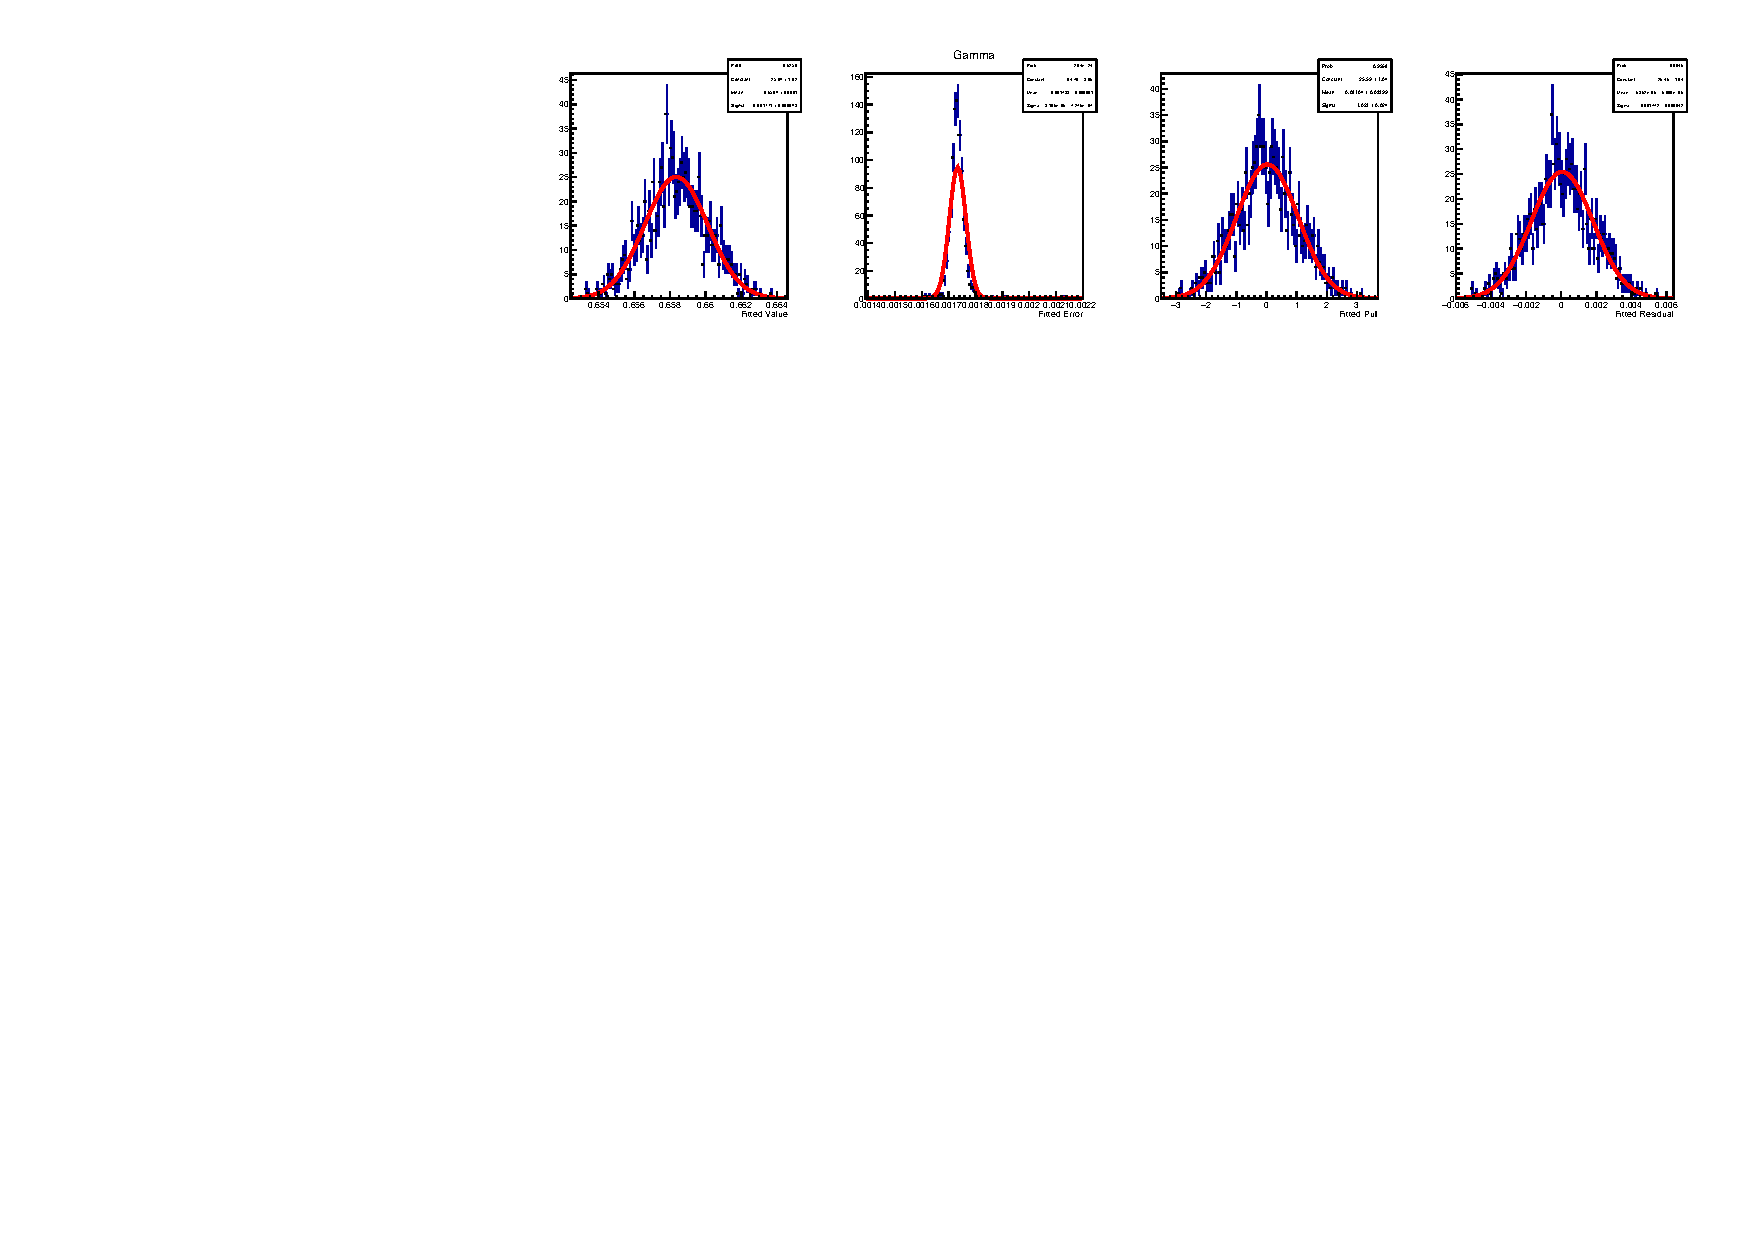
\includegraphics[width=0.9\textwidth]{AA-Appdx-toytagger/figs/1DPullPlot_Gamma_SSbarAccAsymmFloatDMGammaConstrAllSamplesToyTagger.pdf}
        \end{center}
        \vspace{-2mm}
        \caption{Distributions of the fitted value, error, pull and residual for the main parameters ($S_f$, $S_{\bar f}$, $\Delta m$, and $\Gamma$, from top to bottom) fitted on bootstrapped Monte Carlo samples with a toy tagger. Each distribution is fitted with a Gaussian function. Pulls and residuals are computed by taking the Monte Carlo generation value as reference.}
        \label{fig:mc_bootstrap_decay_toytagger}
\end{figure}
